\title{Seismic imaging using the oriented wave equation}
\author{Sergey Fomel}

\maketitle

\begin{abstract}
Seismic waves propagate not only in space and time but also in
direction. The mathematical description of waves propagating in phase
space (space-time-direction) is provided by the oriented wave
equation. I derive this equation and apply it for seismic images using
synthetic and field data examples. The advantages of imaging in the
phase-space domain include the ease of separating different wave
components, the ease of forming angle gathers, and the ease of
handling seismic anisotropy. The disadvantage is the computational
expense of extra dimensions.
\end{abstract}

\section{Introduction}

Imaging in the angle domain has become a recurrent theme in the recent
research on seismic imaging. Accounting for the illumination (wave scattering)
angles provides an illumination compensation in Kirchhoff migration
\cite[]{SEG-1999-13581361,SEG-1999-13621365,SEG-2002-11881191,SEG-2003-09210924}.
Formulating the migration operator directly in the angle coordinates leads to
a powerful imaging method with the ability to handle multiple-path
arrivals~\cite[]{SEG-1998-1538,SEG-2002-11961199,GEO68-01-02320254}.  It is also
possible to extract angle-domain common-image gathers from the output of
wave-equation (do\-wnward extrapolation) imaging
\cite[]{SEG-1999-08240827,GEO67-03-08830889,SEG-2002-13601363,GEO68-03-10651074}.

Studying the problem of multiple-arrival traveltime computation,
\cite{pnas,jcp} realized that the regularity of the phase space,
previously explored in the theoretical studies of the asymptotic wave
propagation \cite[]{maslov}, can be used for constructing an efficient numerical
algorithm.  The algorithm is based on a finite-difference discretization of
the set of specially constructed static partial differential equations
(``escape equations'') for the single-valued phase-space traveltime and
location functions. The algorithm of \cite{pnas} serves as a fast
alternative to tracing multiple rays from subsurface imaging point locations
for common-angle Kirchhoff-style imaging.  However, its connection with the
wave-equation methods is not immediately apparent.

In this paper, I extend the theory of the phase-space computations to handle
the wave extrapolation problem. Applying a simple Huygens-principle
construction, I derive a linear partial differential equation that describes
the wave propagation effects in the phase space, where propagating waves are
assigned not only with the time and space coordinates but also with
orientation directions. The oriented wave equation complements the previously
found set of escape equations. It belongs to the transport type and possesses
other attractive theoretical properties. This equation can form the
theoretical basis for angle-domain seismic imaging methods.

\section{Traveltimes and waves in the physical space}


To derive the oriented wave equation, I follow the analogy with the
conventional wave equation operating in the physical space. The first step is
to establish a connection between the traveltime and wave descriptions. In an
isotropic medium, the traveltime $T(\mathbf{x},\mathbf{y})$ from source
$\mathbf{y}$ to a physical point $\mathbf{x}$ is governed by the eikonal
equation
\begin{equation}
  \label{eq:eikonal}
  \left|\nabla_x T\right|^2 = n^2(\mathbf{x})\;, 
\end{equation}
where $n(\mathbf{x})$ is the slowness at $\mathbf{x}$. Let us consider the
problem of extrapolation the wavefield recorded on the surface of the Earth to
some subsurface location. The Huygens principle implies that the continued
wavefield is a superposition of waves from the surface sources. We can express
this superposition formally as
\begin{equation}
\label{eq:cont}
W^{(\pm)}(\mathbf{x},t) = \int\limits_{\partial \mathcal{D}} 
A(\mathbf{x},\mathbf{y})\,
\widehat{W}\left(\mathbf{y},t \mp T(\mathbf{x},\mathbf{y})\right)\,
\mathbf{d y}\;,
\end{equation}
where $\mathbf{y}$ is a point on the surface $\partial \mathcal{D}$, $t$ is
time, $\widehat{W}$ is the surface wavefield, $W$ is the wavefield in the
subsurface $\mathbf{x} \in \mathcal{D}$, and $A$ is the appropriate amplitude
function.  The $\pm$ sign corresponds to the two possible wave extrapolation
schemes: waves traveling inside or outside $\mathcal{D}$. The sign defines the
time delay of the secondary sources on the surface.

The integral representation~(\ref{eq:cont}) is commonly associated with the
high-frequency asymptotic solution of the wave equation and involves
additional filtering to balance the spectra of $W$ and $\widehat{W}$
\cite[]{norm}. In the high-frequency regime, it is equally possible to use it
to derive the wave equation. Start by rewriting equation~(\ref{eq:cont}) in
the frequency domain:
\begin{equation}
\label{eq:contw}
\mathcal{W}^{(\pm)}(\mathbf{x},\omega) = \int\limits_{\partial \mathcal{D}} 
A(\mathbf{x},\mathbf{y})\,
\widehat{\mathcal{W}}\left(\mathbf{y},\omega\right)\,
e^{\mp i \omega\,T(\mathbf{x},\mathbf{y})}\,
\mathbf{d y}\;,
\end{equation}
where $\omega$ is the temporal frequency, and $\mathcal{W}$ is the Fourier
transform of $W$. Differentiating both sides of equation~(\ref{eq:contw}) with
respect to the spatial coordinates $\mathbf{x}$ and retaining only the terms
of the highest order in $\omega$, we obtain
\begin{equation}
\label{eq:nabla}
\nabla \mathcal{W}^{(\pm)} = \mp i \omega\,
\int\limits_{\partial \mathcal{D}} 
\nabla_{\mathbf{x}} T\,A(\mathbf{x},\mathbf{y})\,
\widehat{\mathcal{W}}\left(\mathbf{y},\omega\right)\,
e^{\mp i \omega\,T(\mathbf{x},\mathbf{y})}\,
\mathbf{d y} + \ldots
\end{equation}
Repeated differentiation produces
\begin{equation}
\label{eq:nabla2}
\nabla^2 \mathcal{W}^{(\pm)} = - \omega^2\,
\int\limits_{\partial \mathcal{D}} 
\left|\nabla_{\mathbf{x}} T\right|^2\,A(\mathbf{x},\mathbf{y})\,
\widehat{\mathcal{W}}\left(\mathbf{y},\omega\right)\,
e^{\mp i \omega\,T(\mathbf{x},\mathbf{y})}\,
\mathbf{d y} + \ldots
\end{equation}
According to the eikonal equation~(\ref{eq:eikonal}), the term
$\left|\nabla_{\mathbf{x}} T\right|^2$ does not depend on $\mathbf{y}$ and can
be taken out of the integral sign. The final result is the celebrated wave
equation, commonly used in many different seismic imaging algorithms:
\begin{equation}
\label{eq:nabla}
\nabla^2 \mathcal{W} 
= - \omega^2\,n^2(\mathbf{x})\,\mathcal{W}(\mathbf{x},\omega) 
+ \ldots
\end{equation}
This simplified derivation highlights the formal connection between
traveltimes (wavefronts) and waves in the high-frequency asymptotic
description of the wave propagation.

\section{Traveltimes and waves in the phase space}
A major problem with the integral wavefield
continuation~(\ref{eq:cont}-\ref{eq:contw}) follows from the fact that, in
complex media, the traveltime $T(\mathbf{x},\mathbf{y})$ can take multiple
values because of the possible multiplicity of ray paths between $\mathbf{x}$
and $\mathbf{y}$. The remedy is to rewrite the wave continuation integral in
the angle coordinates \cite[]{SEG-1998-1538}, as follows:
\begin{equation}
\label{eq:pscont}
  \mathcal{W}^{(\pm)}(\mathbf{x},\omega) = 
  \int\limits_{|\mathbf{p}|=n(\mathbf{x})} 
  \widehat{A}(\mathbf{x},\mathbf{p})\,
  \widehat{\mathcal{W}}\left(\widehat{\mathbf{y}}(\mathbf{x},\mathbf{p}),
  \omega\right)\,
e^{\mp i \omega\,\widehat{T}(\mathbf{x},\mathbf{p})}\,\mathbf{d p}\;.
\end{equation}
Here $\widehat{\mathbf{y}}$ and $\widehat{T}$ are the escape location and the
escape time, uniquely defined by the initial location $\mathbf{x}$ and the
initial direction $\mathbf{p} = \nabla_x T$. They correspond to the location
and traveltime of the ray started at $\mathbf{x}$ and traced in the initial
direction $-\mathbf{p}$ at the ray intersection with the surface $\partial
\mathcal{D}$.  By virtue of ray tracing, the escape functions are strictly
single-valued under the assumption of differentiable slowness $n(\mathbf{x})$.
The integral in equation~(\ref{eq:pscont}) is connected with the integral in
equation~(\ref{eq:contw}) via a change of variables. The change of variables
from $\mathbf{p}$ to $\mathbf{y}$ is possible only when the two-way traveltime
function $T(\mathbf{x},\mathbf{y})$ is single-valued \cite[]{GEO52-07-09430964}.

\cite{pnas} derive the following set of partial differential equations
for describing the wavefront propagation in the phase space:
\begin{equation}
\label{eq:esct}
\mathbf{p} \cdot \nabla_{\mathbf{x}} \widehat{T}  + 
n(\mathbf{x})\,\nabla n \cdot \nabla_{\mathbf{p}} \widehat{T} + n^2(\mathbf{x})
= 0
\end{equation}
\begin{eqnarray}
\label{eq:escy}
  \mathbf{p} \cdot \nabla_{\mathbf{x}} \widehat{\mathbf{y}}  + 
n(\mathbf{x})\,\nabla n \cdot \nabla_{\mathbf{p}} \widehat{\mathbf{y}}
& = & 0 \\
\label{eq:escp}
  \mathbf{p} \cdot \nabla_{\mathbf{x}} \widehat{\mathbf{p}}  + 
n(\mathbf{x})\,\nabla n \cdot \nabla_{\mathbf{p}} \widehat{\mathbf{p}}
& = & 0
\end{eqnarray}
The escape equations~(\ref{eq:esct}-\ref{eq:escp}) lift the eikonal
equation~(\ref{eq:eikonal}) from the physical space $\mathbf{x}$ to the
higher-dimensional phase space $\{\mathbf{x},\mathbf{p}\}$.  They are linear,
transport (convection-type) equations, assuming only single-valued solutions
and suitable for a fast numerical computation. The computation produces
surface arrivals simultaneously from all possible subsurface locations and all
possible initial directions \cite[]{jcp}.

Figure~\ref{fig:symes5} shows an example output of the multiple-arrival
computation algorithm. The 2-D slowness model has a smooth slow region
surrounded by fast regions. This causes five distinct arrivals for both point
sources and plane-wave sources located at the surface. Figure~\ref{fig:slices}
displays horizontal slices from the actual computational output: the solutions
of the escape equations. The multi-valued traveltime function for each
individual source can be extracted from these solutions by simple
interpolation.

%% \sideplot{symes5}{width=\columnwidth}{Multiple-arrival traveltimes. Left:
%%   wavefronts extracted for a point source at the surface. Right: wavefronts
%%   extracted for a plane-wave source at the surface. The slowness model is
%%   shown in the background.}  \sideplot{slices}{width=\columnwidth}{Horizontal
%%   slices out of the phase-space multiple-arrival solution. The slices
%%   correspond to 1.8~km depth in Figure~\ref{fig:symes5}. Left: escape
%%   location. The curve shows the part of the solution corresponding to the
%%   point source result in the left plot of Figure~ \ref{fig:symes5}. Right:
%%   escape direction. The curve shows the part of the solution corresponding to
%%   the plane source result in the right plot of Figure~ \ref{fig:symes5}. Five
%%   branches of the solution are identified by projecting the curves to the
%%   horizontal axes.}

To establish the path from traveltimes to wavefields in the phase space, I
separate the integrand of equation~(\ref{eq:pscont}) and call it an
\emph{oriented wave}:
\begin{equation}
\label{eq:ow}
\mathcal{V}^{(\pm)}(\mathbf{x},\mathbf{p},\omega) = 
  \widehat{A}(\mathbf{x},\mathbf{p})\,
  \widehat{\mathcal{W}}\left(\widehat{\mathbf{y}}(\mathbf{x},\mathbf{p}),
  \omega\right)\,e^{\mp i \omega\,\widehat{T}(\mathbf{x},\mathbf{p})}
\end{equation}
Differentiating equation~(\ref{eq:ow}) with respect to both phase-space
components $\mathbf{x}$ and $\mathbf{p}$ and retaining only the terms with the
highest order of frequency $\omega$, we obtain 
\begin{eqnarray}
  \label{eq:psnabla1}
  \nabla_{\mathbf{x}} \mathcal{V}^{(\pm)} & = & 
  \mp i \omega\,\nabla_{\mathbf{x}} \widehat{T} \mathcal{V}^{(\pm)} + \ldots
  \\
  \label{eq:psnabla2}
  \nabla_{\mathbf{p}} \mathcal{V}^{(\pm)} & = & 
  \mp i \omega\,\nabla_{\mathbf{p}} \widehat{T} \mathcal{V}^{(\pm)} + \ldots 
\end{eqnarray}
Equations~(\ref{eq:psnabla1}-\ref{eq:psnabla2}) can be combined with the help
of the escape equation~(\ref{eq:esct}) to produce the following equation
formally independent of the traveltime:
\begin{equation}
  \label{eq:owew}
  \mathbf{p} \cdot \nabla_{\mathbf{x}} \mathcal{V}^{(\pm)} +
  n(\mathbf{x})\,\nabla n \cdot \nabla_{\mathbf{p}} \mathcal{V}^{(\pm)}
  = \pm i \omega\,n^2(\mathbf{x})\,
\mathcal{V}^{(\pm)}(\mathbf{x},\mathbf{p},\omega) + \ldots
\end{equation}
Equation~(\ref{eq:owew}) is the oriented wave equation: the analog of the wave
equation for propagating oriented waves in the phase space. After the inverse
Fourier transform, it takes the following form in the original time domain:
\begin{equation}
  \label{eq:owe}
  \boxed{
\mathbf{p} \cdot \nabla_{\mathbf{x}} V^{(\pm)} +
  n(\mathbf{x})\,\nabla n \cdot \nabla_{\mathbf{p}} V^{(\pm)} 
  = \pm n^2(\mathbf{x})\,\frac{\partial V^{(\pm)}}{\partial t}\;.}
\end{equation}
The oriented wave $\mathcal{V}$ ``knows'' not only its position in space
$\mathbf{x}$ but also its directional orientation $\mathbf{p}$. According to
equation~(\ref{eq:pscont}), the usual propagating wave $\mathcal{W}$ is simply
a superposition of waves oriented in all possible directions or, in other
words, a projection of the oriented waves from the phase space to the
observable physical space.  Additional weighting may be required to account
for the amplitude and spectrum differences. The dimensionality analysis and
the analogy with the Weyl angular-spectrum representation \cite[]{santo} suggest
the balanced connection
\begin{equation}
  \label{eq:v2w}
  \mathcal{W}(\mathbf{x},\omega) \sim i\,\omega\,\int 
  \mathcal{V}(\mathbf{x},\mathbf{p}_y,\omega)\,
  \frac{d\,\mathbf{p}_y}
  {\sqrt{n^2(\mathbf{x})-\mathbf{p}_y \cdot \mathbf{p}_y}}\;.
\end{equation}
In equation~(\ref{eq:v2w}), the direction vector $\mathbf{p}$ is 
partitioned as $\{\mathbf{p}_y,p_z\}$ with
\[
p_z=\sqrt{n^2(\mathbf{x})-\mathbf{p}_y \cdot \mathbf{p}_y}\;,
\]
and the integration over a sphere in~(\ref{eq:pscont}) is replaced with
integration over a plane.

\section{Oriented waves in layered media}

%\inputdir{Math}

The connection between physical and oriented waves is particularly clear in
the case when the slowness function changes with only one spatial coordinate.
Let $\mathbf{x}=\{\mathbf{y},z\}$. If the slowness $n(\mathbf{x})$ is a
function of $z$, we can make a change of variables in equation~(\ref{eq:owe})
from $p_z$ to $q = \sqrt{s^(z)-p_z^2}$ and then restrict $q$ to comply with
the eikonal equation~(\ref{eq:eikonal}). This results in the simplified
equation
\begin{equation}
  \label{eq:owevz}
\sqrt{n^2(z)- \mathbf{p}_y \cdot \mathbf{p}_y}\,
\frac{\partial V^{(\pm)}}{\partial z} +
\mathbf{p}_y \cdot \nabla_y \partial V^{(\pm)}
= \pm n^2(z)\,\frac{\partial V^{(\pm)}}{\partial t}\;.
\end{equation}
In the frequency-wavenumber domain, the solution to equation~(\ref{eq:owevz})
for propagating waves in the $z$-direction is given by the simple phase-shift
operator:
\begin{equation}
  \label{eq:oweps}
  \widetilde{\mathcal{V}}^{(\pm)}(z+\Delta z,\mathbf{k}_y,\mathbf{p}_y,\omega) =
  \widetilde{\mathcal{V}}^{(\pm)}(z,\mathbf{k}_y,\mathbf{p}_y,\omega)\,
  e^{\,k_z(\mathbf{k}_y,\mathbf{p}_y,\omega)\,\Delta z}\;,
\end{equation}
where 
\begin{equation}
  \label{eq:owekz}
  k_z(\mathbf{k}_y,\mathbf{p}_y,\omega) = 
  \frac{\pm \omega\,n^2(z) + \mathbf{k}_y \cdot \mathbf{p}_y}
  {\sqrt{n^2(z)-\mathbf{p}_y \cdot \mathbf{p}_y}}
\end{equation}
The meaning of equation~(\ref{eq:owekz}) becomes clearer when we notice that
substituting $\mathbf{p}_y= \pm \nabla_y T = \mp \mathbf{k}_y/\omega$ reduces
it to the expression
\begin{equation}
  \label{eq:wekz}
  k_z(\mathbf{k}_y,\omega) = \pm \omega\,n(z)\,
  \sqrt{1-\frac{\mathbf{k}_y \cdot \mathbf{k}_y}{n^2(z)\,\omega^2}}\;,
\end{equation}
and equation~(\ref{eq:oweps}) becomes the familiar phase-shift continuation in
the physical frequency-wavenumber domain \cite[]{GEO43-07-13421351}. Similarly,
the inverse transformation for the constant-slowness case
\begin{equation}
  \label{eq:owest}
  \pm \omega(\mathbf{k}_y,\mathbf{p}_y) = \frac{k_z\,\sqrt{n^2-\mathbf{p}_y
      \cdot \mathbf{p}_y} - \mathbf{k}_y \cdot \mathbf{p}_y}{n^2}
\end{equation}
reduces to the familiar frequency-wavenumber relationship
\cite[]{GEO43-01-00230048}
\begin{equation}
  \label{eq:west}
  \omega(\mathbf{k}_y) = \pm \mbox{sign}{(k_z)}\frac{\sqrt{k_z^2 + 
      \mathbf{k}_y \cdot \mathbf{k}_y}}{n}\;.
\end{equation}
Equation~(\ref{eq:owekz}) decomposes these physical-space-domain expressions
into their individual phase-space components. Figure~\ref{fig:ostolt} shows
how the Stolt hyperbola~(\ref{eq:west}) gets composed from individual
phase-space planes~(\ref{eq:owest}). Figure~\ref{fig:omig} displays the
kinematic impulse response of the constant-velocity zero-offset migration to
show how, in the simplest of all possible situations, the energy gets
distributed from the physical space to the phase space. This distribution is
additionally demonstrated in Figure~\ref{fig:ogaz} by creating a decomposition
of the impulse response by partial stacking in the phase-space domain.

\begin{figure}[htbp]
\centering
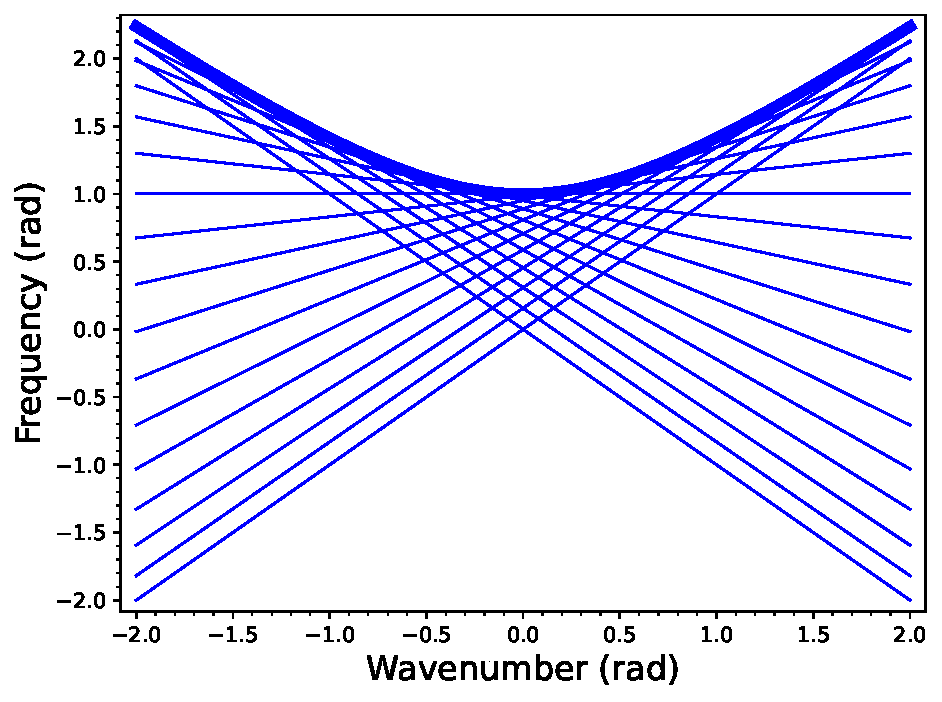
\includegraphics[width=\columnwidth]{Math/Fig/ostolt.pdf}
\caption{Stolt's frequency-wavenumber hyperbola
  is the envelop of frequency-wavenumber planes from oriented plane waves.}
\label{fig:ostolt}
\end{figure}

\begin{figure}[htbp]
\centering
\includegraphics[width=0.8\columnwidth]{Math/Fig/omig.pdf}
\caption{Kinematic impulse response of the
  constant-velocity zero-offset phase-space migration.}
\label{fig:omig}
\end{figure}

%\sideplot{ostolt}{width=\columnwidth}{Stolt's frequency-wavenumber hyperbola
%  is the envelop of frequency-wavenumber planes from oriented plane waves.}
%\sideplot{omig}{width=0.8\columnwidth}{Kinematic impulse response of the
%  constant-velocity zero-offset phase-space migration.}
%% \sideplot{ogaz}{width=0.8\columnwidth,height=1.6\columnwidth}{Decomposition of
%%   the constant-velocity zero-offset migration impulse response by partial
%%   phase-space stacks. Displayed from top to bottom are stacks from
%%   $-60^{\circ}$ to $-30^{\circ}$, $-30^{\circ}$ to $0^{\circ}$ degrees,
%%   $0^{\circ}$ to $30^{\circ}$, and $30^{\circ}$ to $60^{\circ}$.}

Prestack downward continuation of individual phase-space components can be
accomplished by simultaneous continuation of sources and receivers:
\begin{equation}
  \label{eq:owedsr}
  k_z(\mathbf{k}_s,\mathbf{k}_r,\mathbf{p}_s,\mathbf{p}_r,\omega) = 
  \frac{\pm \omega\,n^2(z) + \mathbf{k}_s \cdot \mathbf{p}_s}
  {\sqrt{n^2(z)-\mathbf{p}_s \cdot \mathbf{p}_s}}
  + \frac{\pm \omega\,n^2(z) + \mathbf{k}_s \cdot \mathbf{p}_s}
  {\sqrt{n^2(z)-\mathbf{p}_s \cdot \mathbf{p}_s}}\;,
\end{equation}
Equation~(\ref{eq:owedsr}) is related to the double-square-root method
\cite[]{iei}.

In the 2-D constant-velocity case, it is convenient to express the direction
vectors in terms of angles: 
\begin{equation}
  \label{eq:angles}
p_r + p_s = 2\,n\,\sin{\alpha}\,\cos{\theta}\;;\quad
p_r - p_s = 2\,n\,\cos{\alpha}\,\sin{\theta}\;,  
\end{equation}
where $\alpha$ is the dip angle and $\theta$ is the scattering angle. The
oriented frequency-wavenumber relationship is then
\begin{equation}
  \label{eq:owedsr}
  k_z(k_m,k_h,\alpha,\gamma,\omega) = 
  \frac{\pm 2\,\omega\,n^2 + k_m\,\sin{\alpha}\,\cos{\alpha} +
    k_h\,\sin{\gamma}\,\cos{\gamma}}{\cos^2{\alpha}-\sin^2{\gamma}}\;,
\end{equation}
where $k_m = k_s + k_r$ and $k_h = k_r - k_s$. The time-space-domain analog of
expression~(\ref{eq:owedsr}) corresponds precisely to the constant-velocity
angle-migration Kirchhoff operators \cite[]{paul}.

\section{Discussion}

The oriented wave equation describes wave propagation in the phase space,
where propagating waves are associated not only with time and space
coordinates but also with orientation directions. The ordinary time-and-space
waves are projections from the phase space: a sum of oriented waves from all
possible directions. This concept relates directly to the concept of
angle-domain seismic imaging. It has the following attractive properties:
\begin{itemize}
\item The two directions of wave propagation (up- and down-going waves) are
  explicitly separated by the choice of sign in equation~(\ref{eq:owe}).
\item Equation~(\ref{eq:owe}) is the first-order transport
  (con\-ve\-cti\-on-type) equation, convenient for both mathematical and
  numerical analysis.
\item In the case of lateral velocity variations, equation~(\ref{eq:owe})
  requires the slowness field $n(\mathbf{x})$ to be continuously
  differentiable. This is a reasonable requirement in the seismic imaging
  problem, because it assures the absence of multiple reflections in the
  propagated wavefield.
\item It is possible to extend the oriented wave concept in a straightforward
  way to accommodate the orientation-related effects such as anisotropy and
  vector  wavefield polarization.
\end{itemize}

The practical advantage of the oriented wave approach follows from the fact
that recorded seismic wavefields allow for a sparse representation in the
phase-space domain. The sparseness is easily understood in the case of layered
or constant-velocity media. In the general case, it should be possible to
preserve sparseness in the downward wavefield continuation by decomposing the
wavefield into spatially constrained oriented beams \cite[]{wg}. The oriented
wave equation allows Gaussian beams \cite[]{GEO66-04-12401250} or other sparse
phase-space data representations to be downward continued without
computationally troublesome ray tracing. Exploring this opportunity remains an
open direction for future research.

\bibliographystyle{seg} 
\bibliography{SEP2,SEG,owe}

%%% Local Variables: 
%%% mode: latex
%%% TeX-master: t
%%% TeX-master: t
%%% TeX-master: t
%%% End: 

